\documentclass[UTF8]{ctexart}

\usepackage{amsmath}
\usepackage{subfigure}
\usepackage{hyperref}

\usepackage[graphicx]{realboxes}


\title{Image Caption 学习笔记 Week 2}
\author{高崧淇}
\date{\today}

\begin{document}

\maketitle
\tableofcontents

\section{多模态预训练}

\subsection{简介}
计算机视觉(CV)和自然语言处理(NLP)的研究有着悠久的传统。
计算机视觉研究获取、处理和理解图像的方法,目的是教机器如何看。
而自然语言处理关注以自然语言实现计算机和人类之间交互,即教机器在不同任务中如何阅读并理解文本。
但是将两者结合起来,开发一个可以回答关于图像的任意自然语言问题的计算机视觉系统一直是一个难以解决的目标。
自 2014 年以来,学界在开发视觉语言联合系统方面取得了巨大进展。最开始是从视觉问答 (VQA) 任务入手的,
VQA是一项介于图像理解(CV)和自然语言处理(NLP)的交集任务, 目的是开发出一种系统来回答有关输入图像的特定问题。
问题可以是任意的,它们包含计算机视觉中的许多子问题~\cite{ref1}, {\em e.g.}

\begin{itemize}
    \item[$\bullet$] 图像识别 – 图像里有什么?
    \item[$\bullet$] 目标检测 – 图像里是否有一只猫咪?
    \item[$\bullet$] 属性分类 – 图像里的猫咪是什么颜色的?
    \item[$\bullet$] 场景分类 – 今天是晴天吗?
    \item[$\bullet$] 实例计数 – 图像里有几只猫咪?
\end{itemize}

过去的工作倾向于使用传统神经网络或通过直接使用注意力来进行跨视觉和语言的特征交互,
但是在 2018 年BERT~\cite{ref_bert} 被提出之后,越来越多的工作基于 Transformer实现。
多模态领域的研究人员也立即转向了预训练+微调范式,而不是单任务训练。
因此,VQA 任务逐渐成为了许多多模态任务中的普通 V+L 下游任务,而Image Caption任务也融入到多模态的研究范式中。

\subsection{Oscar}\label{subsec:oscar}
截止目前,coco数据集的上各种方法的BLEU-4排行榜如图~\ref{fig:1},可以看到 Oscar~\cite{ref_oscar} 以41.7的成绩位列第三,其中第一名是序列到序列的方法,
第二名 LEMON 和 Oscar 一样是VLP模型。由此可见,由视觉语言联合预训练的统一架构多模态模型已经在Image Caption领域占据了主导地位。

\begin{figure}
    \centering
    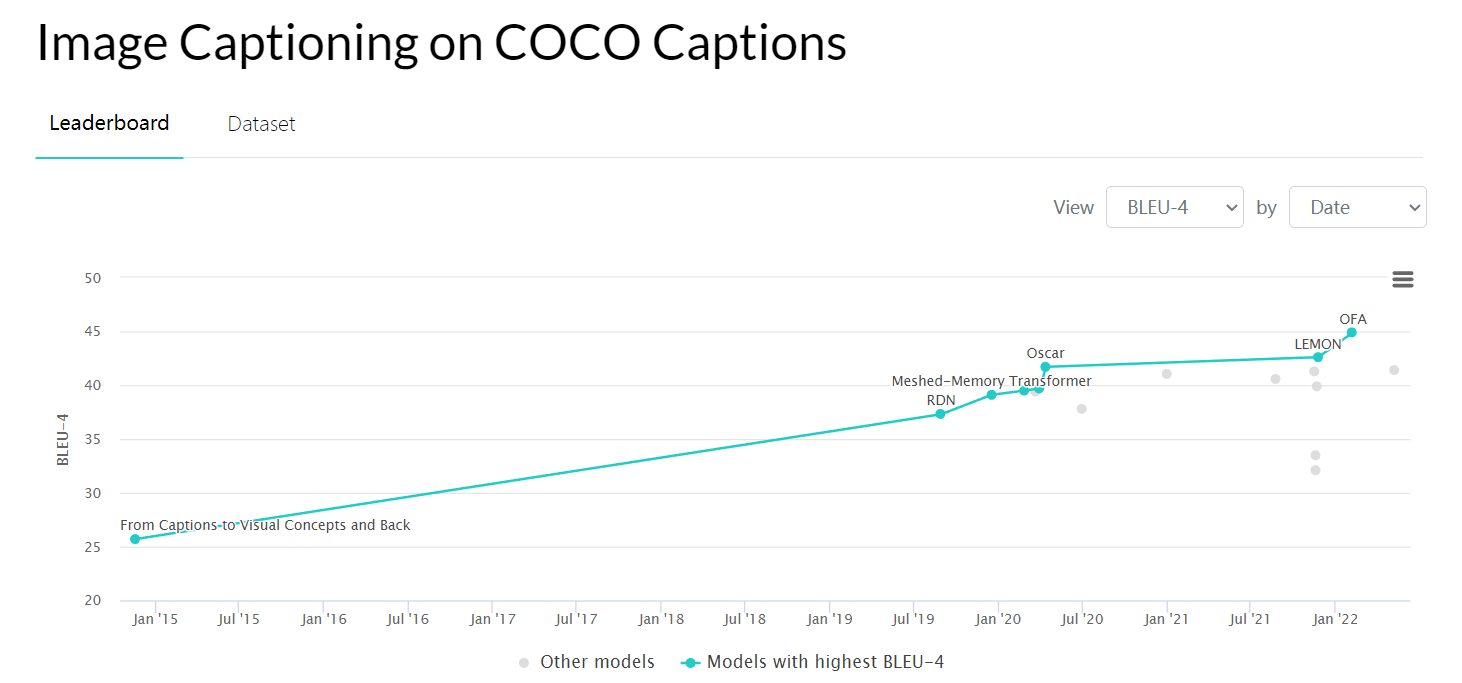
\includegraphics[width=\textwidth]{leader_board}
    \caption{截止目前COCO数据集上的排行榜}
    \label{fig:1}
\end{figure}

\subsection{动机}\label{subsec:motivation}
现存的VLP模型在多数使用场景中只是将文本特征和图像特征简单拼接在一起作为模型的输入以进行预训练,
他们希望借助Transformer的self-attention机制,让模型以一种暴力的手段自我学习达到文本-图像的语义对齐。
Oscar一文则在多模态预训练任务中提出了“锚点”(anchor point)的概念,
作者将从图像中检测到的物体标签用作文本和图像语义对齐学习过程中的“锚点”,更好的对齐语义。

\subsection{预训练}
现存的VLP模型基本都使用$(w, q)$作为输入,而Oscar的输入是一个三元组$(w, q, v)$。其中w是文字序列word tokens的word embedding,
$q$是从图像中检测出来的物体标签所产生的word embedding,
它的作用就是上文提及的“锚点”,$v$是从图中抽取出来的图像特征的集合。整体如图~\ref{fig:2}所示。
$v$的抽取过程由Faster R-CNN完成,由初始的2048维物体特征与6维位置信息组合成一个2054维张量,
再经过一层线性投影得到最终的visual embedding。图像区域对应的物体标签,由Faster R-CNN同时检测出来,并经过BERT Embedding处理,得到$q$。
\begin{figure}
    \centering
    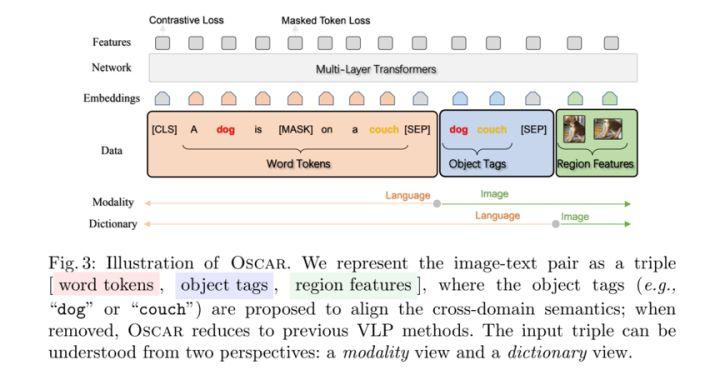
\includegraphics[width=\textwidth]{oscar}
    \caption{Oscar模型示意图}
    \label{fig:2}
\end{figure}

预训练任务
\begin{itemize}
    \item[$1)$] 和BERT类似,随机掩盖掉15\%的单词,并训练模型根据上下文及图片信息预测出Masked Token的能力
    \item[$2)$] 在预训练阶段,以50\%的概率将一个随机的物体标签去替换掉正确的物体标签, 从而生成一些错误的图文序对, 然后训练模型检测是否物体标签和图像特征相匹配的能力:
\end{itemize}

\subsection{效果}
作者为Oscar训练了base和large两个版本,均在各种下游任务上展现了良好的性能,如图~\ref{fig:3}。
\begin{figure}
    \centering
    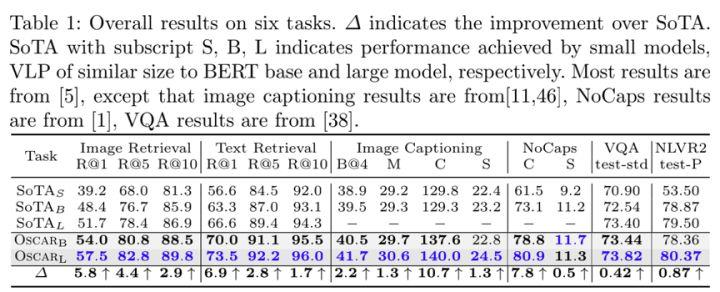
\includegraphics[width=\textwidth]{oscar_performence}
    \caption{Oscar在不同任务上的表现}
    \label{fig:3}
\end{figure}

\section{模型复现}
我在本机部署并修改了组里给出的Image Caption框架。
中间踩坑了一些路径转换,pkl模型加载等问题,总体来说比较顺利(这里要吹一波组里给的框架,比起google开源的一些基于jax的模型的仓库好用太多)。
使用了Show and Tell那篇文章的模型,在batch size开到100的情况下,单个step在两秒左右,




\begin{thebibliography}{8}
    \bibitem{ref1}
    Kafle, Kushal, and Christopher Kanan.
    "Visual question answering: Datasets, algorithms, and future challenges."
    Computer Vision and Image Understanding 163 (2017): 3-20.

    \bibitem{ref_bert}
    Devlin, Jacob, et al. "Bert: Pre-training of deep bidirectional transformers for language understanding." arXiv preprint arXiv:1810.04805 (2018).

    \bibitem{ref_oscar}
    Li, Xiujun, et al. "Oscar: Object-semantics aligned pre-training for vision-language tasks." European Conference on Computer Vision. Springer, Cham, 2020.

\end{thebibliography}

\end{document}
